\documentclass[convert={density=300,outext=.png}]{standalone}
\usepackage{tikz}


%\usetikzlibrary{external}

%\tikzset{external/system call={pdflatex \tikzexternalcheckshellescape 
%-halt-on-error
%                                        -interaction=batchmode 
%                                        -jobname "\image" "\texsource"
%                                        && pdftops -png "\image.png"}}
%\tikzexternalize[shell escape=-enable-write18]

%opening
%\title{}
%\author{}
%\date{}

\begin{document}


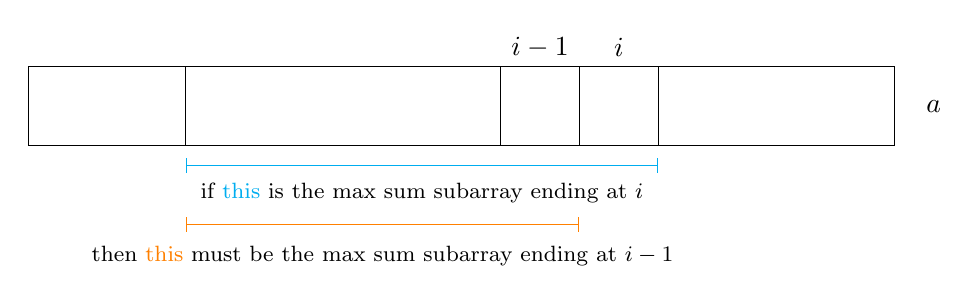
\begin{tikzpicture}

\def\x{0}
\def\y{0}

%\fill (\x + 1, \y + 0) rectangle (\x + 6, \y + 1);

\draw (\x + -1, \y + 0) rectangle (\x + 10, \y + 1);
\draw (\x + 7, \y + 0) -- (\x + 7, \y + 1);
\draw (\x + 6, \y + 0) -- (\x + 6, \y + 1);
\draw (\x + 1, \y + 0) -- (\x + 1, \y + 1);
\draw (\x + 5, \y + 0) -- (\x + 5, \y + 1);

\node at (10.5, 0.5) {$a$};

\node at (\x + 6.5, \y + 1.25) {$i$}; 
\node at (\x + 5.5, \y + 1.25) {$i - 1$}; 

\draw[|-|, cyan] (\x + 1, \y + -0.25) -- (\x + 7, \y + -0.25);

\node at (\x + 4, \y + -0.6) {\footnotesize if {\color{cyan} this} is the max sum subarray ending at $i$};

\draw[|-|, orange] (\x + 1, \y + -1) -- (\x + 6, \y + -1);

\node at (\x + 3.5, \y + -1.4) {\footnotesize then {\color{orange} this} must be the max sum subarray ending at $i - 1$};



%\node at (\x + 3.5, \y + -0.6) {\footnotesize max sum subarray ending at $i - 1$};

% 
% \def\x{-7}
% \def\y{-4}
% 
% \fill[green!50!white] (\x + 6, \y + 0) rectangle (\x + 7, \y + 1);
% 
% \draw (\x + -1, \y + 0) rectangle (\x + 10, \y + 1);
% \draw (\x + 7, \y + 0) -- (\x + 7, \y + 1);
% \draw (\x + 6, \y + 0) -- (\x + 6, \y + 1);
% \draw (\x + 1, \y + 0) -- (\x + 1, \y + 1);
% \draw (\x + 5, \y + 0) -- (\x + 5, \y + 1);
% 
% \node at (\x + 6.5, \y + 1.25) {$i$}; 
% \node at (\x + 5.5, \y + 1.25) {$i - 1$}; 
% 
% 
% \draw[|-|] (\x + 1, \y + -0.25) -- (\x + 6, \y + -0.25);
% 
% \node at (\x + 3.5, \y + -0.6) {\footnotesize max sum subarray ending at $i - 1$};
% 
% 
% 
% \def\x{7}
% \def\y{-4}
% 
% \fill[green!50!white] (\x + 1, \y + 0) rectangle (\x + 6, \y + 1);
% 
% \draw (\x + -1, \y + 0) rectangle (\x + 10, \y + 1);
% \draw (\x + 7, \y + 0) -- (\x + 7, \y + 1);
% \draw (\x + 6, \y + 0) -- (\x + 6, \y + 1);
% \draw (\x + 1, \y + 0) -- (\x + 1, \y + 1);
% \draw (\x + 5, \y + 0) -- (\x + 5, \y + 1);
% 
% \node at (\x + 6.5, \y + 1.25) {$i$}; 
% \node at (\x + 5.5, \y + 1.25) {$i - 1$}; 
% 
% 
% \draw[|-|] (\x + 1, \y + -0.25) -- (\x + 6, \y + -0.25);
% 
% \node at (\x + 3.5, \y + -0.6) {\footnotesize max sum subarray ending at $i - 1$};

\end{tikzpicture}


\end{document}

